\documentclass[GTS.tex]{subfiles}
%\usepackage{amsmath,amssymb}
%\usepackage[utf8]{inputenc}
%\usepackage[spanish]{babel}
%\usepackage[]{graphicx,wrapfig}
%\usepackage{enumerate}
%\usepackage{amsthm}
%\usepackage{tikz-cd}  
%\usetikzlibrary{babel} 
%\usepackage{pgf,tikz}
%\usepackage{mathrsfs}
%\usetikzlibrary{arrows}
%\usetikzlibrary{cd}    
%\usepackage[spanish]{babel}
%\usepackage{fancyhdr}
%\usepackage{titlesec}
%\usepackage{floatrow}    
%\usepackage{makeidx}      
%\usepackage[tocflat]{tocstyle}  
%\usetocstyle{standard} 
%%\usepackage{breqn}
%\usepackage{bm}         
%%\usepackage[sc]{mathpazo}
%%\usepackage{blindtext}
%\usepackage{color}   %May be necessary if you want to color links
%\usepackage{hyperref}
%\hypersetup{colorlinks=true,citecolor=red, linkcolor=blue}
%
%
%\renewcommand{\baselinestretch}{1,4}
%\setlength{\oddsidemargin}{0.25in}
%\setlength{\evensidemargin}{0.25in}
%\setlength{\textwidth}{6in}
%\setlength{\topmargin}{0.1in}
%\setlength{\headheight}{0.1in}
%\setlength{\headsep}{0.1in}
%\setlength{\textheight}{8in}
%\setlength{\footskip}{0.75in}
%
%\newtheorem{teorema}{Teorema}[section]
%\newtheorem{defi}[teorema]{Definición}
%\newtheorem{coro}[teorema]{Corolario}
%\newtheorem{lemma}[teorema]{Lema}
%\newtheorem{ej}[teorema]{Ejemplo}
%\newtheorem{ejs}[teorema]{Ejemplos}
%\newtheorem{observacion}[teorema]{Observación}
%\newtheorem{observaciones}[teorema]{Observaciones}
%\newtheorem{prop}[teorema]{Proposición}
%\newtheorem{propi}[teorema]{Propiedades}
%\newtheorem{nota}[teorema]{Nota}
%\newtheorem{notas}[teorema]{Notas}
%\newtheorem*{dem}{Demostración}
%\newtheorem{ejer}[teorema]{Ejercicio}
%\newtheorem{consec}[teorema]{Consecuencia}
%\newtheorem{consecs}[teorema]{Consecuencias}
%
%\providecommand{\abs}[1]{\lvert#1\rvert}
%\providecommand{\norm}[1]{\lVert#1\rVert}
%\providecommand{\ninf}[1]{\norm{#1}_\infty}
%\providecommand{\numn}[1]{\norm{#1}_1}
%\providecommand{\gabs}[1]{\left|{#1}\right|}
%\newcommand{\bor}[1]{\mathcal{B}(#1)}
%\newcommand{\R}{\mathbb{R}}
%\newcommand{\Z}{\mathbb{Z}}
%\newcommand{\N}{\mathbb{N}}
%\newcommand{\Q}{\mathbb{Q}}
%\newcommand{\C}{\mathbb{C}}
%\newcommand{\Pro}{\mathbb{P}}
%\newcommand{\Tau}{\mathcal{T}}
%\newcommand{\verteq}{\rotatebox{90}{$\,=$}}
%\newcommand{\vertequiv}{\rotatebox{110}{$\,\equiv$}}
%\providecommand{\lrg}{\longrightarrow}
%\providecommand{\func}[2]{\colon{#1}\longrightarrow{#2}}
%\newcommand*{\QED}{\hfill\ensuremath{\blacksquare}}
%\newcommand*\circled[1]{\tikz[baseline=(char.base)]{
%            \node[shape=circle,draw,inner sep=1.5pt] (char) {#1};}}
%\newcommand*{\longhookarrow}{\ensuremath{\lhook\joinrel\relbar\joinrel\rightarrow}}
%
%\newenvironment{solucion}{\begin{trivlist}
%\item[\hskip \labelsep {\textit{Solución}.}\hskip \labelsep]}{\end{trivlist}}
%
%\def\quot#1#2{%
%    \raise1ex\hbox{$#1$}\Big/\lower1ex\hbox{$#2$}%
%}
%
%\makeatletter
%\renewcommand\tableofcontents{%
%  \null\hfill\textbf{\Large\contentsname}\hfill\null\par
%  \@mkboth{\MakeUppercase\contentsname}{\MakeUppercase\contentsname}%
%  \@starttoc{toc}%
%}
%
%\pagestyle{fancy}
%\fancyhf{}
%\rhead{Topología de Superficies (Grado en Matemáticas)}
%\lhead{Curso 2016/2017}
%\cfoot{\thepage}
%
\begin{document}
%
\renewcommand\chaptername{\Huge Tema}

\titleformat{\chapter}[display]
    {\normalfont\huge\bfseries}{\chaptertitlename\ \thechapter}{10pt}{\Huge}
\titlespacing*{\chapter}{0pt}{-1cm}{10pt}
%
%
%
%\tableofcontents


\setcounter{chapter}{3}

\chapter{Cálculo del Grupo Fundamental}

Conocer el grupo fundamental de la circunferencia junto a la herramienta de cálculo que proporciona el teorema de Seifert-Van Kampen permite determinar el grupo fundamental de una gran variedad de ejemplos. Nuestro interés está centrado en las superficies.

\section{Grupo fundamental de $S^1$}

Vamos a empezar recalcando un {\em hecho crucial}. Sea $p\func{\R}{S^1}\mid p(t)=(\cos(2\pi t),\sen(2\pi t))$, entonces $\forall x\in S^1\ \exists$ un abierto $U_x\subseteq S^1$ tal que $p^{-1}(U_x)$ es unión disjunta de abiertos $V_a$, uno por cada $a\in p^{-1}(x)$ y, además para cada $a$
\[
p_a=p_{\big|_{V_a}}\func{V_a}{U_x}
\]
es homeomorfismo.
\begin{defi}
Llamamos \textbf{fibra} de $x$ a $p^{-1}(x)$ y \textbf{cubierta} de $U_x$ a cada $V_a$ (que contiene a $a$).
\end{defi}

Por ejemplo, si $x=(\cos(2\pi t_0),\sen(2\pi t_0))$ con $0\leq t_0 < 1$, entonces la fibra de $x$ la forman los puntos $t_0+2\pi k$ con $k\in \Z$, y si  $U_x =\{y\in S^1; y=(\cos(2\pi t),\sen(2\pi t)); |t-t_0| < \varepsilon\}$ donde $\varepsilon<1-t_0$, las cubiertas que componen  $p^{-1}(U_x)$ son $(2\pi k+t_0-\varepsilon,2\pi k+t_0+\varepsilon)$ con $k\in\Z$.

\definecolor{ffqqqq}{rgb}{1.,0.,0.}
\begin{tikzpicture}[line cap=round,line join=round,>=triangle 45,x=1.0cm,y=1.0cm]
\clip(0,-1.1) rectangle (12,1.5);
\draw(10.,0.) circle (1.cm);
\draw (2.,0.)-- (7.,0.);
\draw [shift={(10.,0.)},line width=2.pt,color=ffqqqq]  plot[domain=0.49486877921189426:1.1386278121351083,variable=\t]({1.*1.*cos(\t r)+0.*1.*sin(\t r)},{0.*1.*cos(\t r)+1.*1.*sin(\t r)});
\draw [line width=2.pt,color=ffqqqq] (2.5,0.)-- (3.5,0.);
\draw [line width=2.pt,color=ffqqqq] (4.,0.)-- (5.,0.);
\draw [line width=2.pt,color=ffqqqq] (5.5,0.)-- (6.5,0.);
\draw (10.7420476743391841,1.0072827448034072) node[anchor=north west] {$x$};
\draw (7.8,0.7) node[anchor=north west] {$p$};
\draw (10.3,1.4) node[anchor=north west] {$U_x$};
\draw (2.763767502219794,0.014636523006171236) node[anchor=north west] {$t_0-2\pi$};
\draw (4.430320333310567,-0.003577169136897315) node[anchor=north west] {$t_0$};
\draw (5.805454090112242,0.014636523006171236) node[anchor=north west] {$t_0+2\pi$};
\draw (11.,0.5) node[anchor=north west] {\Large{$S^1$}};
\draw (2.,0.6) node[anchor=north west] {\Large{$\mathbb{R}$}};
\begin{scriptsize}
\draw [fill=ffqqqq] (10.6841203828864005,0.7293691121231861) circle (2.5pt);
\draw [fill=ffqqqq] (3.,0.) circle (2.5pt);
\draw [fill=ffqqqq] (4.5,0.) circle (2.5pt);
\draw [fill=ffqqqq] (6.,0.) circle (2.5pt);
\draw[->](7.5,0.2)-- (8.5,0.2);
\end{scriptsize}
\end{tikzpicture}


\begin{lemma}[Lema de Lebesgue] Sea $(X,d)$ un espacio métrico compacto, y $\mathcal{U}$ un recubrimiento por abiertos de $X$. Entonces existe un $\delta>0$ tal que todo subconjunto de $X$ con diámetro menor que $\delta$ está contenido en algún abierto del recubrimiento.
\end{lemma}
\begin{dem}
Como $X$ es compacto, podemos extraer un subrecubrimiento finito $\{A_1,\dots A_n\}\subseteq\mathcal{U}$. Para cada $i\in\{1,\dots n\}$ sea $C_i=X\setminus A_i$, y definimos la función $f\func{X}{\R}$ como
\[
f(x)=\frac{1}{n}\sum_{i=1}^n d(x,C_i)
\]
Dado que $f$ es una función continua en un compacto, alcanza un mínimo $\delta>0$. Ahora, si $Y\subseteq X$ tiene diámetro menor que $\delta$, existe $x_0\in X$ tal que $Y\subseteq B(x_0,\delta)$. Como $f(x)\geq\delta$ debe existir al menos un $i$ de modo que $d(x_0,C_i)\geq\delta$. Pero esto significa que $B(x_0,\delta)\subseteq A_i$, y en particular, $Y\subseteq A_i$. $\QED$
\end{dem}

\begin{teorema}
$\pi_1(S^1,(1,0))\cong\Z$
\end{teorema}

\begin{dem}Consistirá en alcanzar los siguientes objetivos:
\begin{enumerate}
\item[$\circled{1}$] Dados un camino $\alpha\func{I}{S^1}\mid\alpha(0)=x_0$ y $\alpha(1)=x_1$, y cualquier $a\in p^{-1}(x_0)$, $\exists!$ camino $\tilde{\alpha}\func{I}{\R}\mid\tilde{\alpha}(0)=a$ y $p\circ\tilde{\alpha}=\alpha$ ($\Rightarrow \tilde{\alpha}(1)\in p^{-1}(x_1)$) llamado \underline{elevación} de $\alpha$ por $a$. En particular, si $\alpha$ es la aplicación constante $x_0$, $\tilde{\alpha}$ es la constante $a$. Por otro lado, si $\alpha$ es un lazo en $x_0=(1,0)$, entonces $\tilde{\alpha}(1)\in p^{-1}(x_0)\Rightarrow\tilde{\alpha}(1)=a+2\pi k, k\in\Z$. A $k$ se le llama grado de $\alpha$ ($grad(\alpha)=k$).

\begin{figure}[h!]
	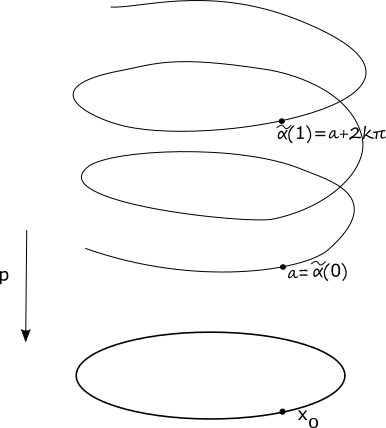
\includegraphics[scale=0.5]{text4479}
\end{figure}

\item[$\circled{2}$] Si $\alpha\sim\beta$ son caminos equivalentes entre $x_0$ y $x_1$, entonces también lo son sus elevaciones por $a$, $\tilde{\alpha}$ y $\tilde{\beta}$. En particular, si $\alpha$ y $\beta$ son lazos en $x_0=(0,1)$ entonces $grad(\alpha)=grad(\beta)$.
\item[$\circled{3}$] Definir
\begin{gather*}
\Phi\func{\pi_1(S^1,x_0)}{\Z}\\
\Phi([\alpha])=grad(\alpha)
\end{gather*}
\item[$\circled{4}$] $\Phi$ es isomorfismo. En particular, $\alpha(t)=e^{2\pi it}$ es un lazo en $S^1$ que representa un generador de $\pi_1(S^1,x_0)$.
\end{enumerate}
Pasamos ahora a demostrar estos puntos, con lo que quedará probado el teorema.
\begin{enumerate}
\item[$\circled{1}$] Sea $\mathcal{U}$ un recubrimiento de $S^1$ por abiertos que admiten cubiertas. Por el lema de Lebesgue existe una partición de $[0,1]$, $0=t_0<t_1<\cdots<t_n=1$,  tal que para todo $i=0,\dots, n-1$ existe $U_i\in\mathcal{U}$ con  $\alpha([t_i,t_{i+1}])\subseteq U_i$. Tenemos $x_0\in U_0$ y sea $V_a$ la cubierta de $U$ con $a\in V_a$. Por ser $p_a$ homeomorfismo podemos definir
\[
\tilde{\alpha}_{\big|{[0,t_1]}}=p_a^{-1}\circ\alpha_{\big|[0,t_1]}.
\]
Ahora $\alpha(t_1)\in U_1$ y si $V_{a_1}$ es la cubierta de $U_1$ con $a_1=\tilde{\alpha}(t_1)\in V_{a_1}$, tomamos
\[
\tilde{\alpha}_{\big|{[t_1,t_2]}}=p_{a_1}^{-1}\circ\alpha_{\big|[t_1,t_2]}.
\]

Siguiendo este proceso, llegamos a construir un camino $\tilde{\alpha}\func{I}{S^1}$ con $\tilde{\alpha}(0)=a$ y $p\circ\tilde{\alpha}=\alpha$. Veamos que es único:\\
Supongamos que $\hat{\alpha}$ es otra elevación que cumple $\hat{\alpha}(0)=a$ y $p\circ\hat{\alpha}=\alpha$. Sea $A=\{t:\tilde{\alpha}(t)=\hat{\alpha}(t)\}$. Se tiene $A\neq\emptyset$ pues $\tilde{\alpha}(0)=\hat{\alpha}(0)=a$. Además, vamos a ver que $A=\overline{A}$. Si $t\in\overline{A}\Rightarrow\exists\ \{t_n\}\subseteq A$ convergiendo hacia $t$. Como $t_n\in A$, $\tilde{\alpha}(t_n)=\hat{\alpha}(t_n)$, y por continuidad $\tilde{\alpha}(t)=\hat{\alpha}(t)\Rightarrow t\in A$.\\
Por último vamos a ver que $A$ es abierto. Sea $t\in A\Rightarrow\tilde{\alpha}(t)=\hat{\alpha}(t)$. Sea $U\in\mathcal{U}$, abierto admitiendo cubiertas, con $\alpha(t)\in U$. Por continuidad $\exists\ \varepsilon>0\mid \alpha((t-\varepsilon,t+\varepsilon))\subseteq U$. Ahora consideramos $\hat{\alpha}((t-\varepsilon,t+\varepsilon))$ y $\tilde{\alpha}((t-\varepsilon,t+\varepsilon))$. Se tiene que ambos están contenidos en $p^{-1}(U)$ y son conexos por ser imagen continua de conexos. Como $p^{-1}(U)$ es unión disjunta de cubiertas, $\hat{\alpha}((t-\varepsilon,t+\varepsilon))$ y $\tilde{\alpha}((t-\varepsilon,t+\varepsilon))$ están contenidos cada uno en una cubierta, pero como además comparten un punto ($\tilde{\alpha(t)}=\hat{\alpha}(t)$), están en la misma, la cual llamaremos $V_{a'}$. Tenemos que $p_{a'}$ es homeomorfismo y $p_{a'}\circ\tilde{\alpha}((t-\varepsilon,t+\varepsilon))=p_{a'}\circ\hat{\alpha}((t-\varepsilon,t+\varepsilon))=\alpha((t-\varepsilon,t+\varepsilon))\Rightarrow\tilde{\alpha}(t')=\hat{\alpha}(t')\ \forall t'\in (t-\varepsilon,t+\varepsilon)\Rightarrow (t-\varepsilon,t+\varepsilon)\subseteq A\Rightarrow t\in int(A)\Rightarrow A$ es abierto. \\

$A\neq\emptyset$, $A$ abierto y cerrado en el espacio conexo $[0,1]\Rightarrow A$ es $[0,1]$.
\item[$\circled{2}$] Supongamos que $\alpha\sim\beta\Rightarrow\exists\ H\func{I\times I}{S^1}$ homotopía relativa a $\{0,1\}$ entre $\alpha$ y $\beta$.

\begin{tikzpicture}[line cap=round,line join=round,>=triangle 45,x=1.0cm,y=1.0cm]
\clip(-2,-0.4) rectangle (13.026666666666669,2.1);
\draw (0.,0.)-- (2.,0.);
\draw [line width=2.8pt] (2.,0.)-- (2.,2.);
\draw (2.,2.)-- (0.,2.);
\draw [line width=2.8pt] (0.,2.)-- (0.,0.);
\draw [->] (2.45,1) -- (3.64,1);
\draw (3.853333333333334,1.3) node[anchor=north west] {\large{$S^1$}};
\draw (0.5,1.3266666666666656) node[anchor=north west] {\large{$I\times I$}};
\draw (2.8,1.5933333333333322) node[anchor=north west] {$H$};
\draw (-0.2,0) node[anchor=north west] {$0$};
\draw (1.8,0) node[anchor=north west] {$1$};
\end{tikzpicture}

Sea $\mathcal{U}$ un recubrimiento de $S^1$ por abiertos admitiendo cubiertas como en $\circled{1}$. Por el lema de Lebesgue existe una partición  de $I\times I$ en cuadrados $R_{ij}$ tal que $\forall R_{ij}\ \exists U_{ij}\in\mathcal{U}$ con $H(R_{ij})\subseteq U_{ij}$. Denotemos por $H_{ij}$ a la restricción $H\big|_{R_{ij}}$.

\begin{tikzpicture}[line cap=round,line join=round,>=triangle 45,x=1.0cm,y=1.0cm]
\clip(-2.966666666666667,-0.1) rectangle (12,3.1);
\draw [line width=1.2pt] (0.,0.)-- (0.,3.);
\draw [line width=1.2pt] (0.,0.)-- (3.,0.);
\draw [line width=1.2pt] (0.,3.)-- (3.,3.);
\draw [line width=1.2pt] (3.,3.)-- (3.,0.);
\draw [line width=1.2pt] (0.9,3.)-- (0.9,2.146666666666665);
\draw [line width=1.2pt] (0.9,2.146666666666665)-- (0.,2.146666666666665);
\draw [line width=1.2pt] (2.1533333333333333,3.)-- (2.1533333333333333,2.146666666666665);
\draw [line width=1.2pt] (2.1533333333333333,2.146666666666665)-- (3.,2.146666666666665);
\draw [line width=1.2pt] (0.,0.9066666666666658)-- (0.9,0.9066666666666658);
\draw [line width=1.2pt] (0.9,0.9066666666666658)-- (0.9,0.);
\draw [line width=1.2pt] (2.1533333333333333,0.)-- (2.1533333333333333,0.9066666666666658);
\draw [line width=1.2pt] (2.1533333333333333,0.9066666666666658)-- (3.,0.9066666666666658);
\draw [line width=1.2pt,dash pattern=on 3pt off 3pt] (0.9,2.146666666666665)-- (0.9,0.9066666666666658);
\draw [line width=1.2pt,dash pattern=on 3pt off 3pt] (0.9,2.146666666666665)-- (2.1533333333333333,2.146666666666665);
\draw [line width=1.2pt,dash pattern=on 3pt off 3pt] (2.1533333333333333,2.146666666666665)-- (2.1533333333333333,0.9066666666666658);
\draw [line width=1.2pt,dash pattern=on 3pt off 3pt] (2.1533333333333333,0.9066666666666658)-- (0.9,0.9066666666666658);
\draw (0.1,2.8266666666666644) node[anchor=north west] {$R_{n1}$};
\draw (2.2,2.8) node[anchor=north west] {$R_{nn}$};
\draw (0,0.6533333333333329) node[anchor=north west] {$R_{11}$};
\draw (0.2,2) node[anchor=north west] {$\vdots$};
\draw (2.5,2) node[anchor=north west] {$\vdots$};
\draw (1.2,2.75) node[anchor=north west] {$\cdots$};
\draw (1.2,0.55) node[anchor=north west] {$\cdots$};
\draw (1.2,2) node[anchor=north west] {$\ddots$};
\draw (2.1,0.6) node[anchor=north west] {$R_{1n}$};
\end{tikzpicture}

Vamos a definir una homotopía $\widetilde{H}\func{I\times I}{\R}$ entre $\tilde{\alpha}$ y $\tilde{\beta}$.

\begin{tikzpicture}[line cap=round,line join=round,>=triangle 45,x=1.0cm,y=1.0cm]
\clip(-0.5,-0.5) rectangle (5.5,1.5);
\draw [line width=2.pt] (0.,1.)-- (0.,0.);
\draw (0.,0.)-- (5.,0.);
\draw [line width=2.pt] (5.,0.)-- (5.,1.);
\draw (0.,1.)-- (5.,1.);
\draw [line width=1.2pt] (1.,0.)-- (1.,1.);
\draw (2.,0.)-- (2.,1.);
\draw (4.,0.)-- (4.,1.);
\draw (-0.2,0) node[anchor=north west] {$x_0$};
\draw (5.013333333333334,0.13333333333333336) node[anchor=north west] {$x_1$};
\draw (0.92,0.08) node[anchor=north west] {$t_1$};
\draw (0.1,0.76) node[anchor=north west] {$R_{11}$};
\draw (1.1,0.72) node[anchor=north west] {$R_{12}$};
\draw (4.1,0.7466666666666668) node[anchor=north west] {$R_{1n}$};
\draw (0.2,1.52) node[anchor=north west] {\small{$\{t_1\}\times [0,t_1]$}};
\draw (2.8266666666666667,0.68) node[anchor=north west] {$\cdots$};
\draw (2.8266666666666667,0) node[anchor=north west] {$\alpha$};
\begin{scriptsize}
\draw [fill=black] (0.,0.) circle (1.5pt);
\draw [fill=black] (5.,0.) circle (1.5pt);
\draw [fill=black] (1.,0.) circle (1.5pt);
\end{scriptsize}
\end{tikzpicture}

Sea $V_a$ la cubierta de $U_{11}$ conteniendo a $a$. Elegimos $\widetilde{H}_{11}=p^{-1}_a\circ H_{11}$. En particular, como $H_{11}(0,s)=x_0$ y $H_{11}(t,0)=\alpha(t)\ \forall t,s\in[0,1]$, se sigue por la unicidad de elvaciones que $\widetilde{H}_{11}(0,s)=a$ y $\widetilde{H}_{11}(t,0)=\tilde{\alpha}(t)\ \forall t,s\in[0,1]$.

Sea ahora $V_{a_1}$ la cubierta de $U_{12}$ con $a_1=\tilde{\alpha}(t_1)\in V_{a_1}$. Se define $\widetilde{H}_{12}=p^{-1}_{a_1}\circ H_{12}$. Hay que ver que $\widetilde{H}_{11}$ y $\widetilde{H}_{12}$ coinciden en $R_{11}\cap R_{12}=\{t_1\}\times[0,t_1]$. Esto es cierto, pues las restricciones $\widetilde{H}_{11}$ y $\widetilde{H}_{12}$ a dicha intersección son elevaciones del camino $\gamma\func{[0,t_1]}{S^1}$ dado por $\gamma(s)=H(t_1,s)$ que valen $\tilde{\alpha}(t_1)$ para $s=0$, por lo que la unicidad de elevaciones nos da $\widetilde{H}_{11}=\widetilde{H}_{12}$ sobre $R_{11}\cap R_{12}$. Ahora seguimos inductivamente hasta conseguir una aplicación continua
\[
\widetilde{H}_1\func{\bigcup_{k=1}^n R_{1k}=[0,1]\times[0,t_1]}{\R}
\]
tal que $\widetilde{H}_1(t,0)=\tilde{\alpha}(t)$, $\widetilde{H}_1(0,s)=\widetilde{H}_{1n}(0,s)=a$ y  $\widetilde{H}_1(1,s)=\widetilde{H}_{11}(1,s)=\tilde{\alpha}(1)$ para $t\in [0,1]$ y $s\in[0,t_1]$. En la última igualdad se usa de nuevo la unicidad de elevación de caminos y el hecho de que $H(1,s)=\alpha(1)=x_1\ \forall s\in[0,t_1]$. 

Ahora se va subiendo inductivamente nivel a nivel hasta conseguir una aplicación continua $\widetilde{H}\func{I\times I}{\R}$ con $\widetilde{H}(t,0)=\tilde{\alpha}(t)$, $\widetilde{H}(0,s)=a$ y $\widetilde{H}(1,s)=\tilde{\alpha}(1)\ \forall s,t\in[0,1]$. Más aún, como
$\widetilde{H}(0,1)=a$, $\widetilde{H}(t,1)$ es una elevación de $H(t,1)=\beta(t)$, que empieza en $a$ y por ello es $\tilde{\beta}$. Se ha probado así que $\tilde{\alpha}\sim\tilde{\beta}$.

\item[$\circled{3}$] La buena definición de $\Phi$ es una consecuencia inmediata de $\circled{2}$.

\item[$\circled{4}$] Veamos primero que $\Phi$ es homomorfismo, esto es:
\[
\Phi([\alpha][\beta])=\Phi([\alpha*\beta])=grad(\alpha*\beta)=grad(\alpha)+grad(\beta).
\]

Esto es consecuencia de la igualdad $\widetilde{\alpha*\beta}=\tilde{\alpha}*\tilde{\beta}$ donde $\tilde{\beta}$ es la elevación de $\beta$ por $\tilde{\alpha}(1)$. Obsérvese que, por la elección de $\tilde{\beta}$, existe la yuxtaposición de $\tilde{\alpha}$ y $\tilde{\beta}$. Además, la compatibilidad de esta yuxtaposición con la composición nos da
\[
p\circ(\tilde{\alpha}*\tilde{\beta})=p\circ\tilde{\alpha}*p\circ\tilde{\beta}=\alpha*\beta.
\]

Por unicidad de elevaciones esto implica que la elevación de $\alpha*\beta$ empezando por $\tilde{\alpha}(0)$ es $\widetilde{\alpha*\beta}=\tilde{\alpha}*\tilde{\beta}$. Así que
\[
\widetilde{\alpha*\beta}(1)=\tilde{\alpha}*\tilde{\beta}(1)=\tilde{\beta}(1)=grad(\beta)+\tilde{\alpha}(1)=grad(\beta)+grad(\alpha).
\]


Veamos ahora que $\Phi$ es isomorfismo.
\begin{itemize}
\item $\Phi$ sobre:\\
Dado $k\in\Z$ sea, $\alpha_k(t)=(\cos(2\pi kt),\sen(2\pi kt))$. Entonces la elevación $\tilde{\alpha}_k$ empezando en $0\in\R$ es el camino $\tilde{\alpha}_k(t)=2\pi k t$ y por tanto
\[
grad(\alpha_k)=\tilde{\alpha}_k(1)=2\pi k.
\]

\item $\Phi$ inyectiva:\\
$\Phi([\alpha])=0\Rightarrow grad(\alpha)=0$. Por tanto, $\tilde{\alpha}$ es un lazo en $0\Rightarrow [\tilde{\alpha}]=0\in\pi_1(\R,0)=\{0\}$. Así que, para $p_*\func{\pi_1(\R,0)}{\pi_1(S^1,(1,0))}$ tenemos $p_*[\tilde{\alpha}]=[p\circ\tilde{\alpha}]=[\alpha]\Rightarrow 0=[\alpha]$. $\QED$
\end{itemize}
\end{enumerate}
\end{dem}

\vspace{0.2cm}

\begin{nota}
El resultado es válido sea cual sea el punto sobre el que se calcula el grupo fundamental de $S^1$.
\end{nota}

%\newpage

\begin{nota}
Hay otros muchos ejemplos de lo que hemos llamado ``hecho crucial", a partir de los cuales se desarrolla la llamada \underline{teoría de cubiertas}:
\begin{itemize}
\item[$\circled{A}$] Sea $p\func{\R^2}{S^1\times S^1}$ (toro) dada por $p(t,s)=((\cos(2\pi t), \sen(2\pi t)),(\cos(2\pi s), \sen(2\pi s)))$
\begin{figure}[h!]
	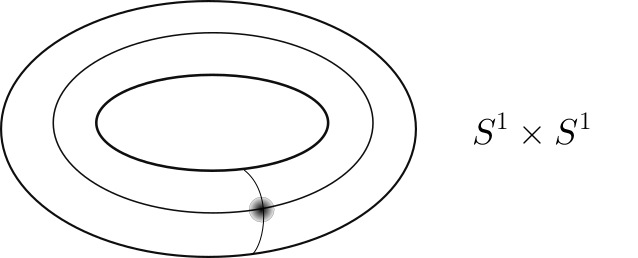
\includegraphics[scale=0.5]{path4172}
\end{figure}

\begin{tikzpicture}[line cap=round,line join=round,>=triangle 45,x=1.0cm,y=1.0cm]
\draw [color=black,, xstep=2.0cm,ystep=2.0cm] (-1.5933333333333337,-2.066666666666667) grid (13.74,5.36);
\clip(-1.5933333333333337,-2.066666666666667) rectangle (13.74,3.5);
\draw [fill=black,fill opacity=0.09] (4.,2.) circle (0.38256444627742925cm);
\draw [fill=black,fill opacity=0.09] (4.,0.) circle (0.4009433321001306cm);
\draw [fill=black,fill opacity=0.09] (6.,2.) circle (0.4013864859597433cm);
\draw [fill=black,fill opacity=0.09] (6.,0.) circle (0.410798680080104cm);
\draw [fill=black,fill opacity=0.09] (8.,2.) circle (0.4133870932780679cm);
\draw [fill=black,fill opacity=0.09] (8.,0.) circle (0.42921116274186405cm);
\draw [->] (2.,0.) -- (1.9933333333333332,1.);
\draw [->] (4.,0.) -- (3.9933333333333336,1.);
\draw [->] (6.,0.) -- (6.006666666666667,1.);
\draw [->] (8.,0.) -- (8.006666666666668,1.);
\draw [->] (2.,0.) -- (2.993333333333333,0.);
\draw [->] (4.,0.) -- (5.02,0.);
\draw [->] (6.,0.) -- (7.006666666666667,0.);
\draw [->] (2.,2.) -- (2.993333333333333,1.986666666666667);
\draw [->] (4.,2.) -- (5.02,1.986666666666667);
\draw [->] (6.,2.) -- (7.006666666666667,1.986666666666667);
\draw [->] (4.,2.) -- (4.006666666666667,2.96);
\draw [->] (6.,2.) -- (5.993333333333334,2.92);
\draw [->] (8.,2.) -- (8.913333333333334,1.986666666666667);
\draw [->] (8.,2.) -- (7.993333333333334,2.84);
\draw [->] (8.,0.) -- (8.98,0.);
\draw [->] (8.,0.) -- (8.02,-1.1333333333333335);
\draw [->] (6.,0.) -- (6.006666666666667,-1.12);
\draw [->] (4.,0.) -- (3.9933333333333336,-1.146666666666667);
\draw [line width=2.pt] (2.,2.)-- (8.,2.);
\draw [line width=2.pt] (2.,2.)-- (2.,0.);
\draw [line width=2.pt] (8.,2.)-- (8.,0.);
\draw [line width=2.pt] (2.,0.)-- (8.,0.);
\draw [line width=2.pt] (4.,2.)-- (4.,0.);
\draw [line width=2.pt] (6.,2.)-- (6.,0.);
\draw [line width=2.pt] (2.,2.)-- (0.833333333333333,2.);
\draw [line width=2.pt] (2.,0.)-- (1.0466666666666664,0.);
\draw [line width=2.pt] (2.,0.)-- (2.,-1.);
\draw [line width=2.pt] (4.,0.)-- (4,-1);
\draw [line width=2.pt] (6.,0.)-- (6.,-1.);
\draw [line width=2.pt] (8.,0.)-- (8.0,-1);
\draw [line width=2.pt] (8.,0.)-- (8.8,0.);
\draw [line width=2.pt] (8.,2.)-- (8.8,2);
\draw [line width=2.pt] (8.,2.)-- (8,2.8);
\draw [line width=2.pt] (6.,2.)-- (6,2.8);
\draw [line width=2.pt] (4.,2.)-- (4.,2.8);
\draw [line width=2.pt] (2.,2.)-- (2,2.8);
\draw (-1,2) node[anchor=north west] {\LARGE{$\R^2$}};
\draw (1.5,1.186666666666667) node[anchor=north west] {$b$};
\draw (3.5,1.146666666666667) node[anchor=north west] {$b$};
\draw (5.5,1.1333333333333335) node[anchor=north west] {$b$};
\draw (7.5,1.146666666666667) node[anchor=north west] {$b$};
\draw (2.8066666666666666,2.4666666666666672) node[anchor=north west] {$a$};
\draw (4.873333333333334,2.44) node[anchor=north west] {$a$};
\draw (6.833333333333334,2.44) node[anchor=north west] {$a$};
\draw (2.833333333333333,0) node[anchor=north west] {$a$};
\draw (4.873333333333334,0.) node[anchor=north west] {$a$};
\draw (6.886666666666667,1.8133333333333337) node[anchor=north west] {$a$};
\draw (6.886666666666667,0) node[anchor=north west] {$a$};
\draw (8.2,3.013333333333334) node[anchor=north west] {$Cubiertas$};
\end{tikzpicture}

Vemos en el plano las cubiertas del entorno abierto indicado en la figura.
\vspace{0.2cm}

\item[$\circled{B}$] $S^2\longrightarrow\Pro_2(\R)$
\begin{figure}[h!]
	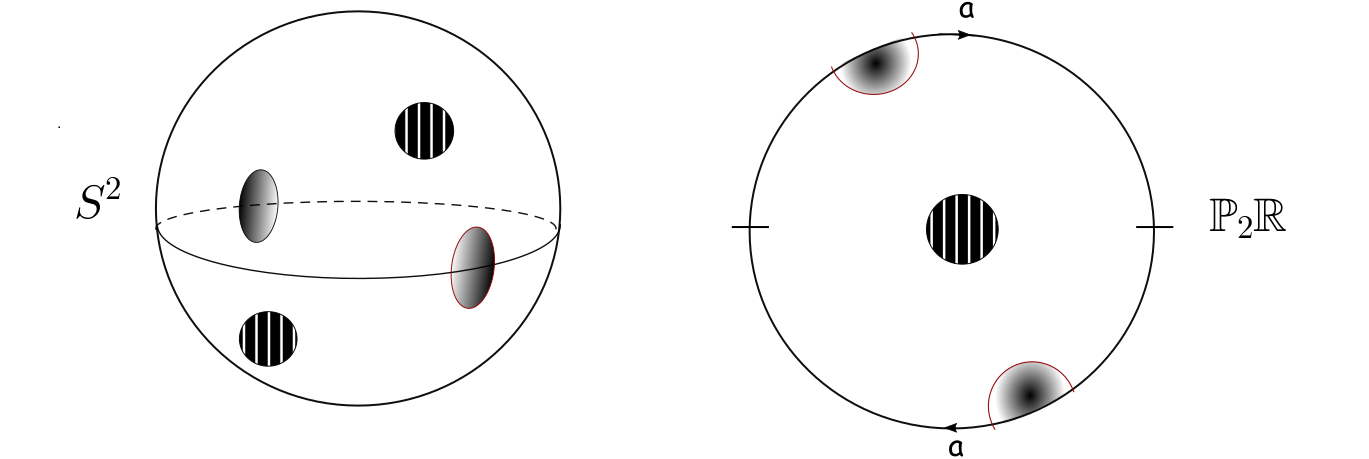
\includegraphics[scale=0.3]{text7103}
	
Vemos en la esfera las dos cubiertas de los abiertos de $\Pro_2\R$.
\end{figure}\
\end{itemize}
\end{nota}

%\vspace{0.2cm}

\section{Aplicaciones}

\begin{teorema}[\textbf{Teorema de no retracción}] No existe retracción de $B^2$ sobre $S^1$.
\end{teorema}
\begin{dem}
$\boxed{RA}$ Supongamos que $\exists\ r\func{B^2}{S^1}$ retracción $\Rightarrow r\circ i=Id_{S^1}$ con $i:S^1\longhookarrow B^2$ la inclusión. Entonces, como $B^2$ es contráctil

\[
\begin{tikzcd}
\Z\cong\pi_1(S^1,x_0)\arrow[r, "i_*"]\arrow[rr, "r_*\circ i_*(r\circ i)_*=Id_*=Id", bend right=-15] & \pi_1(B^2,x_0)=\{1\} \arrow[r, "r_*"] & \pi_1(S^1,x_0)\cong\Z \\
\end{tikzcd}
\]

Pero esto implica que $Id_\Z$ es el homomorfismo trivial, lo cual es una contradicción. $\QED$
\end{dem}

\begin{prop} Sea $f\func{B^2}{\R^2}$, entonces $\exists y\mid f(y)=0$ ó $z\mid f(z)=\lambda z, \lambda>0$.
\end{prop}
\begin{dem}
Sea $g\func{B^2}{\R^2}$ definida como

\[
g(x)=\begin{cases}
(2||x||-1)x-(2-2||x||)f\left(\frac{x}{||x||}\right) & \text{si  } ||x||\geq\frac{1}{2}\\
-f(4||x|| x) & \text{si  } ||x||\leq\frac{1}{2}
\end{cases}
\]

Si $g(x)\neq 0\ \forall x$ se puede definir $h\func{B^2}{S^1}$ por $h(x)=\dfrac{g(x)}{||g(x)||}$. En ese caso, si $||x||=1$, $h(x)=x\Rightarrow h$ sería retracción de $B^2$ sobre $S^1$, lo cual es una contradicción con el teorema anterior. Por lo tanto, $\exists x_0\mid g(x_0)=0$.
\begin{itemize}
\item Si $||x_0||\leq\frac{1}{2}\Rightarrow -f(4||x_0||x_0)=0\Rightarrow f(y)=0$ en $y=4||x_0||x_0$.
\item Si $||x_0||\geq\frac{1}{2}\Rightarrow (2||x||-1)x_0-(2-2||x_0||)f\left(\dfrac{x_0}{||x_0||}\right)=0\Rightarrow f\left(\dfrac{x_0}{||x_0||}\right)=\dfrac{2||x_0||-1}{2-2||x_0||}x_0$. Si tomamos $z=\frac{x_0}{||x_0||}$, llegamos a que
\[
f(z)=\dfrac{||x_0||(2||x_0||-1)}{2-2||x_0||}z=\lambda z \mbox{    para } \lambda=\dfrac{||x_0||(2||x_0||-1)}{2-2||x_0||}>0.
\]
 $\QED$
\end{itemize}
\end{dem}

\vspace{0.2cm}

\begin{prop} Sea $f\func{B^2}{\R^2}$, entonces $\exists$ punto fijo $f(x)=x$ o existe $z\in S^1 \mid f(z)=\lambda z, \lambda>1$.
\end{prop}
\begin{dem}
Supongamos que $f(x)\neq x\ \forall x$. Sea $h\func{B^2}{\R^2}\mid h(x)=f(x)-x$. Entonces $h(x)\neq 0$ y por la proposición anterior, $\exists z\in S^1\mid h(z)=\mu z$ con $\mu>0$, es decir, $f(z)-z=\mu z\Rightarrow f(z)=(1+\mu)z$. Basta tomar $\lambda=1+\mu$. $\QED$
\end{dem}

\vspace{0.2cm}

\begin{teorema}[\textbf{Punto fijo de Brouwer}] Toda $f\func{B^2}{B^2}$ tiene un punto fijo.
\end{teorema}
\begin{dem}
Sea $f\func{B^2}{B^2\subseteq\R^2}$ y supongamos que no tiene ningún punto fijo. Por la proposición anterior, $\exists z\in S^1\mid f(z)=\lambda z$ con $\lambda>1$. Por lo tanto, $||f(z)||=\lambda||z||=\lambda>1$, pero $f(z)\in B^2\Rightarrow||f(z)||\leq 1$, luego hemos llegado a una contradicción. $\QED$
\end{dem}

\newpage 

\begin{teorema}
Todo polinomio $p(z)=a_n z^n+\cdots +a_0$ en $\C$ tiene al menos una raíz.
\end{teorema}
\begin{dem}
En primer lugar definimos $f_n\func{S^1}{S^1}$ como $f_n(z)=z^n$. Obsérvese que $z^n=e^{2\pi nti}=\cos(2\pi nt)+i\sen(2\pi nt)$. De esta forma, el homomorfismo inducido por $f_n$,
\[
f_{n*}\func{\pi_1(S^1,(1,0))}{\pi_1(S^1,(1,0))}\\
\]
lleva el generador $[\alpha]$ representado por $\alpha(t)=e^{2\pi it}$ en la clase de $\alpha_n(t)=e^{2\pi i nt}$ cuyo grado es $n$. Así que $f_{n*}[\alpha]=[\alpha_n]=n[\alpha]$.\\
Ahora pasamos a razonar por reducción al absurdo. Supongamos que $p(z)\neq 0\ \forall z\in\C$. Podemos suponer que $p(z)$ es mónico, pues en caso contrario bastaría con dividir por el término líder. Es decir, vamos a trabajar con $p(z)=z^n+\cdots + a_0$. Sea $M=\max\{1,|a_{n-1}|+\dots +|a_0|\}$. Si $|z|\geq M$, entonces $|z|^j\leq |z|^{n-1}$ para $j\leq n-1$. Además,
\[
|a_{n-1}z^{n-1}+\cdots +a_0|\leq |a_{n-1}||z|^{n-1}+\cdots +|a_0|\leq (|a_{n-1}|+\dots +|a_0|)|z|^{n-1}\leq M|z|^{n-1}\leq|z|^n.
\]
Definimos ahora las homotopías $F\func{S^1\times I}{S^1}$ y $G\func{S^1\times I}{S^1}$ de la siguiente forma
\[
F(z,t)=\frac{p(Mtz)}{|p(Mtz)|}\quad G(z,t)=\frac{H(z,t)}{|H(z,t)|},
\]
donde $H\func{\C\times I}{\C}$ es la función $H(z,t)=z^n+t(a_{n-1}z^{n-1}+\cdots +a_0)$. Se tiene que $F$ es continua porque suponemos $p(z)\neq 0\ \forall z\in\C$. La continuidad de $G$ es inmediata pues el denominador no se anula nunca. En efecto, al ser $|z|\geq M$
\begin{gather*}
H(z,t)=0\Rightarrow z^n+t(a_{n-1}z^{n-1}+\cdots +a_0)=0\Rightarrow \\
z^n=-t(a_{n-1}z^{n-1}+\cdots +a_0)\Rightarrow |z|^n=t|a_{n-1}z^{n-1}+\cdots +a_0|
\end{gather*}
Pero esto significaría que para $0<t<1$, $|z|^n<|a_{n-1}z^{n-1}+\cdots +a_0|\leq|z|^n$, con lo que hemos llegado a una contradicción. Observemos ahora lo siguiente
\begin{gather*}
F(z,0)=\frac{p(0)}{|p(0)|}=1\ (cte)\qquad F(z,1)=\frac{p(Mz)}{|p(Mz)|}\\
G(z,0)=\frac{z^n}{|z|^n}=z^n=f_n(z)\quad G(z,1)=\frac{p(Mz)}{|p(Mz)|}
\end{gather*}
Por transitividad de la relación de homotopía $cte\simeq f_n(z)$. Este resultado nos conduce, considerando el camino $\gamma(t)=H((1,0),t)$ al siguiente diagrama
\[
\begin{tikzcd}
\pi_1(S^1,(1,0)) \ar[r, "f_{n*} "]\arrow[d,"cte_* "'] & \pi_1(S^1,(1,0))\\
\pi_1(S^1,q)\arrow[ur,"\gamma_\sharp "',"\cong"]
\end{tikzcd}
\]
Pero esto es una contradicción porque $f_{n*}\neq 0$, y $cte_*$ es el homomorfismo trivial. $\QED$
\end{dem}

\begin{ejer}
Probar que si identificamos dos puntos de $S^2$, el espacio cociente $X$ tiene grupo fundamental no trivial.
\end{ejer}
\begin{solucion}Si el grupo fundamental de $X$ fuese trivial y nos fijamos en la circunferencia $S^1$ en trazo grueso tenemos que $X$ se retrae sobre $S^1$ (ver dibujo).
\begin{figure}[h!]
	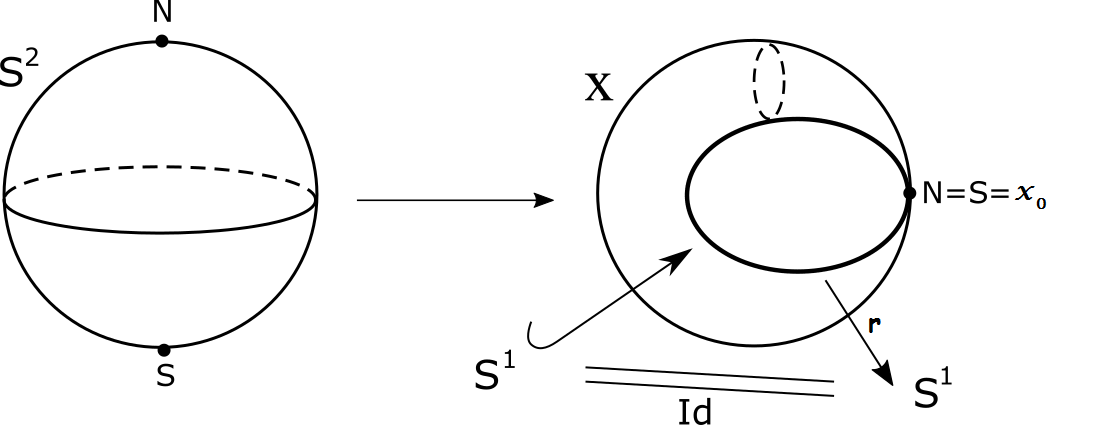
\includegraphics[scale=0.3]{bitmap}
\end{figure}
\[
\begin{tikzcd}
\Z\cong\pi_1(S^1,x_0)\arrow[r,"i_* "] \arrow[rr,"(r\circ i)_*=Id_*=Id",bend left=10] &  \pi_1(X,x_0)\cong\{1\}\ar[r, "r_* "] & \pi_1(S^1,x_0)\cong\Z\\
\end{tikzcd}
\]
Ello implicaría que la identidad de $\Z$ sería el homomorfismo nulo, lo que es una contradicción. \qed
\end{solucion}

\begin{ejer}
Probar que $S^1$ es retracto del toro $S^1\times S^1$ pero no de deformación.
\end{ejer}
\begin{solucion}
Es obvio que la proyección
\begin{gather*}
\quad r:S^1\times S^1\longrightarrow S^1\times\{y_0\}\cong S^1\\
(x,y)\longmapsto (x,y_0)
\end{gather*}
es una retracción. Pero no existe una retracción con deformación $r$. Si exitiera tendríamos $r\circ i=Id_{S^1}$ y $i\circ r\overset{H}{\simeq}Id_{S^1\times S^1}$. Tomando $\gamma=H((1,0),t)$ llegaríamos al siguiente diagrama conmutativo:
\[
\begin{tikzcd}
\pi_1(S^1\times\{y_0\},(x_0,y_0))\cong\Z\ar[dr, "i_*"]\\
\Z\times\Z\cong\pi_1(S^1\times S^1,(x_0,y_0)) \ar[r, "(i\circ r)_* "]\arrow[u,"r_* "']\ar[d,"Id_*=Id"] & \pi_1(S^1\times S^1,(x_0,y_0))\cong\Z\times\Z\\
\Z\times\Z\cong\pi_1(S^1\times S^1,(x_0,y_0))\arrow[ur,"\gamma_\sharp "',"\cong"]
\end{tikzcd}
\]
De este diagrama se deduce que $(i\circ r)_*=i_*\circ r_*$ es un isomorfismo y por tanto $r_*$ sería un homomorfismo inyectivo $\varphi\func{\Z\times\Z}{\Z}$, que no puede existir. En efecto, si $\varphi(1,0)=\lambda\neq 0$ y $\varphi(0,1)=\mu\neq 0$, entonces
\[
\varphi(\mu,-\lambda)=\mu\varphi(1,0)-\lambda\varphi(0,1)=\mu\lambda-\lambda\mu=0. 
\]
\qed
\end{solucion}

\end{document}